\atstartofhistorysection
\section[Un peu d’histoire : le Napier Nomad]{Un peu d’histoire :\onlyamphibook{\\} Le Napier Nomad}
\label{ch_histoire_nomad}\index{Napier Nomad (moteur)}

À la fin de la seconde guerre mondiale, le gouvernement britannique émet un appel d’offres pour le développement d’un moteur aéronautique de \SI{6000}{ch} à très haute efficacité, pour encourager le développement d’appareils militaires et civils. Le motoriste anglo-saxon \textit{Napier \& Son} engage alors des recherches qui donneront naissance à un engin curieux et édifiant : le \textit{Napier Nomad}.

\index{Diesel!moteur}\index{temps moteur!deux temps}\index{injection directe}\index{reactivite@réactivité d’un moteur}\index{moteur!réactivité}\index{refroidissement!intermédiaire}\index{intercooling}\index{turbopropulseur}
Construit à partir d’un moteur à douze cylindres Diesel à deux temps et injection directe, le \textit{Nomad} est aussi doté de tous les éléments d’un turbopropulseur. Pour augmenter la pression et la température auxquelles se fait l’apport de chaleur, les deux ensembles sont montés \emph{en série}, mais pour permettre une grande efficacité à tous les régimes, chacun entraîne l’une des deux hélices contra-rotatives (figures~\ref{fig_napier_i_circuit} et~\ref{fig_napier_i_photos}). Enfin, pour permettre d’atteindre de hautes puissances et d’augmenter la réactivité dans tout le domaine de vol, un système de refroidissement intermédiaire et une réchauffe sont mis en place. Le résultat : un époustouflant et rocambolesque assemblage mécano-thermique évoquant le fantasme débridé d’ingénieurs thermodynamiciens en quête d’efficacité.

	\onlyframabook{\begin{figure}}
	\onlyamphibook{\begin{figure}[htc]}%handmade
		\begin{center}
			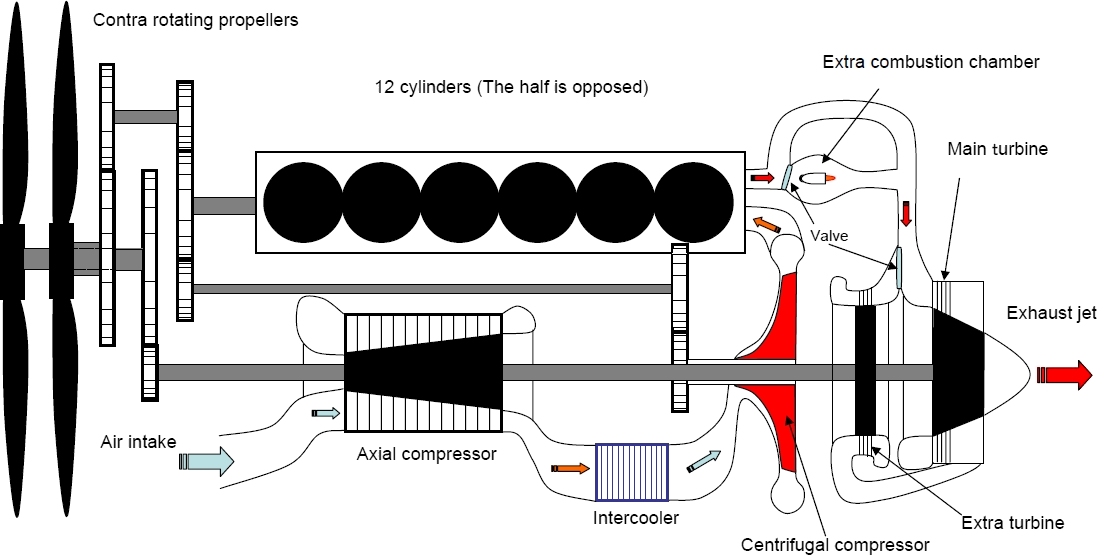
\includegraphics[width=12cm]{images/napier_nomad_i_3.png}
			\supercaption{Schéma de principe du circuit thermodynamique du \textit{Napier Nomad I}. L’arbre de la turbomachine et celui du Diesel alimentent chacun une hélice. Pourtant, les deux ensembles sont montés en série : l’air circule d’abord dans les compresseurs, puis dans les cylindres, puis dans la ou les turbines. La puissance du moteur, comme c’est l’usage en 1950, est contrôlée avec une seule manette de commande mécanique !}%
				{\wcfile{NomadSchematic 185kBpng360kB.png}{schéma} par les utilisateurs$\cdot$rices Commons \wcun{Tataroko-common}{Tataroko-common}, \wcun{Aaa3-other}{Aaa3-other} \& \wcun{Nimbus227}{Nimbus227} (\pd)}
			\label{fig_napier_i_circuit}
		\end{center}
	\end{figure}
	
	\onlyframabook{\begin{figure}}
	\onlyamphibook{\begin{figure}[htc]}%handmade
		\begin{center}
			\onlyframabook{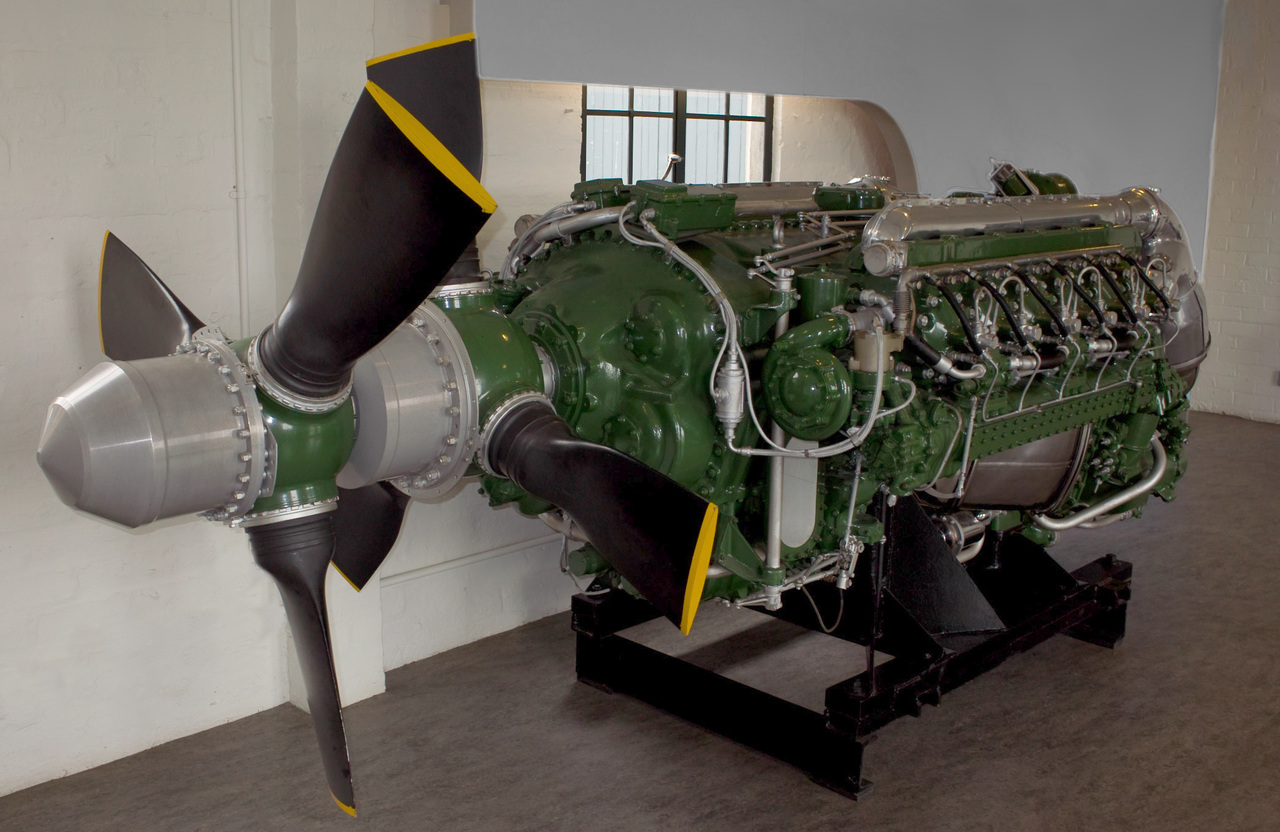
\includegraphics[height=0.395\textwidth]{images/napier_nomad_i_1.jpg}
			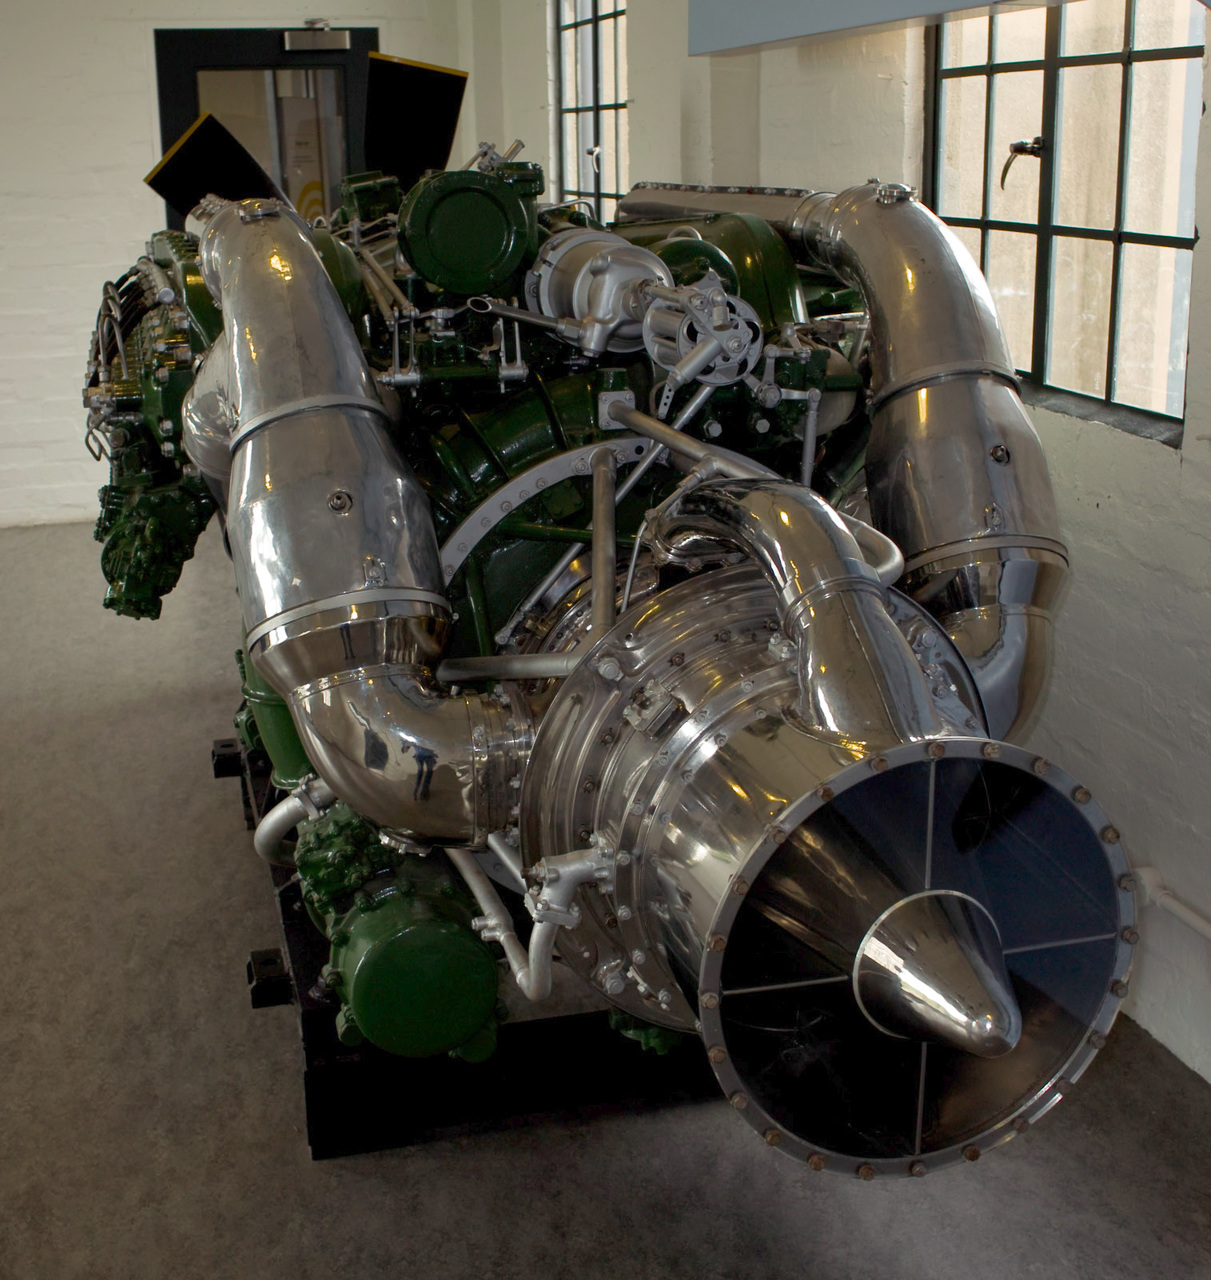
\includegraphics[height=0.395\textwidth]{images/napier_nomad_i_2.jpg}}%
			\onlyamphibook{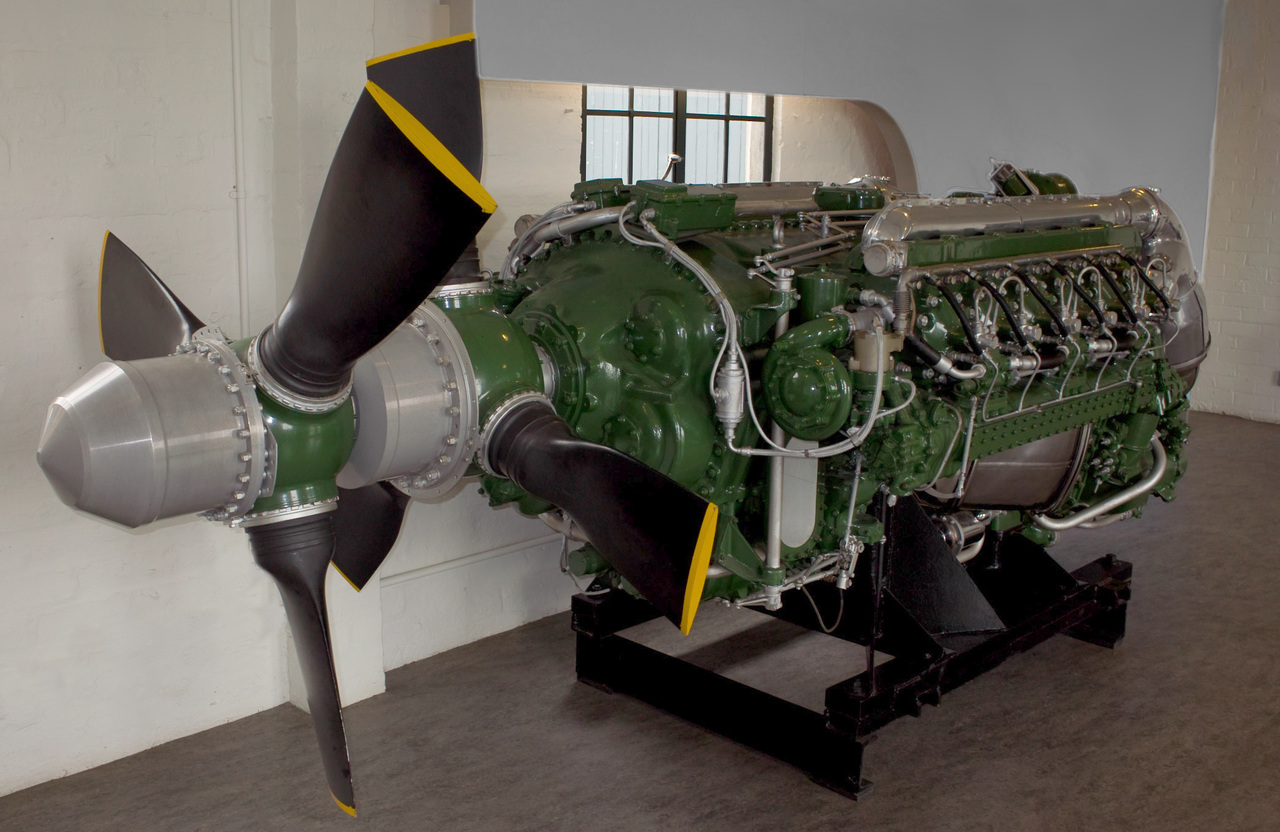
\includegraphics[width=8cm]{images/napier_nomad_i_1.jpg}
			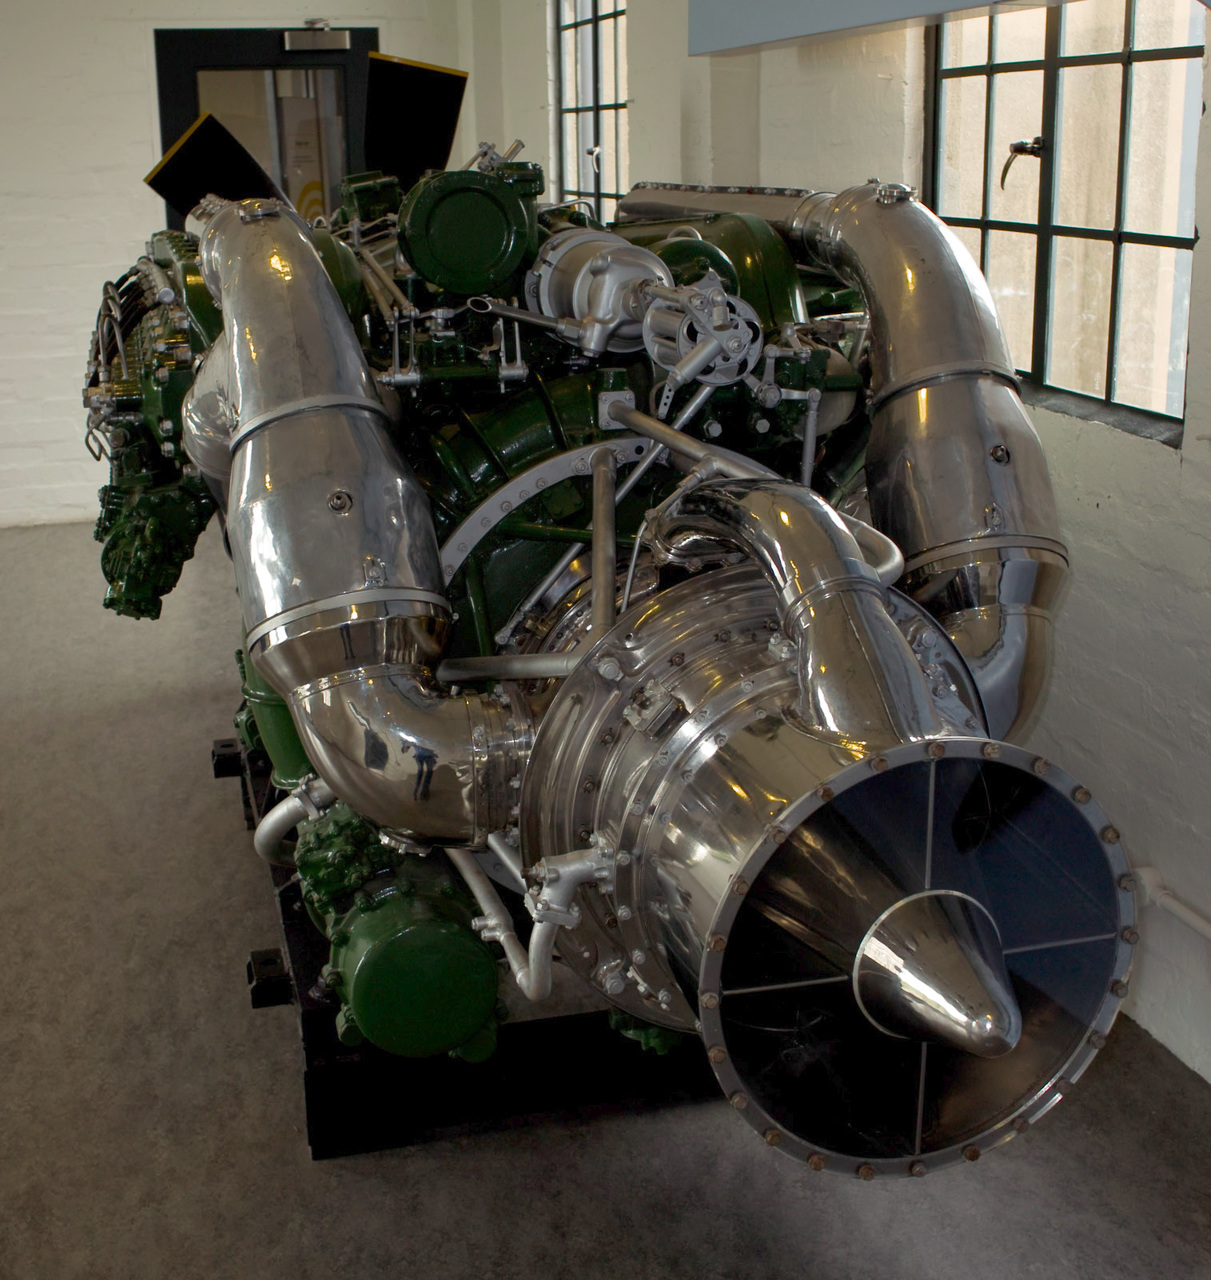
\includegraphics[width=8cm]{images/napier_nomad_i_2.jpg}}
			\supercaption{Le prototype du \textit{Napier Nomad I}. La cylindrée est de \SI{40}{\liter} et le poids dépasse 2~\si{tonnes}.}%
				{Images retouchées à partir de photos (\wcfile{Napier Nomad I East fortune front.jpg}{1} et \wcfile{Napier Nomad I East fortune Rear view.jpg}{2}) \ccbysa par \wcun{Nigel Ish}{Nigel~Ish}}
			\label{fig_napier_i_photos}
		\end{center}
	\end{figure}

\textit{Napier \& Son} rectifie rapidement le tir : le second prototype du moteur, le \textit{\mbox{Nomad II}}, est grandement simplifié. Le refroidissement intermédiaire, la réchauffe et la surcompression centrifuge sont tous abandonnés (\cref{fig_napier_ii_circuit}). Les deux grands ensembles mécaniques, l’un à pistons et l’autre à turbine, sont désormais reliés à la même hélice. Reste la connexion mécanique qui les relie : un ingénieux mais complexe réducteur mécanique et hydraulique à rapport continûment variable permet à chacun de fonctionner à sa vitesse optimale.

	\begin{figure}[htc]%handmade
		\begin{center}
			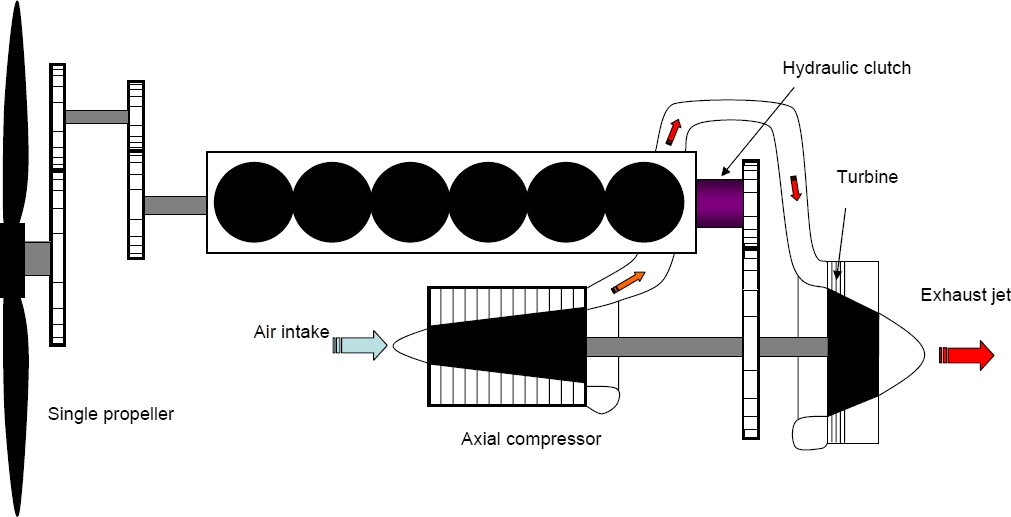
\includegraphics[width=12cm]{images/napier_nomad_ii.png}
			\supercaption{Schéma de principe du circuit thermodynamique du \textit{Napier Nomad II}. Un réducteur mécanique-hydraulique à rapport variable relie les deux ensembles, qui entraînent désormais la même hélice.}%
				{\wcfile{NomadSchematic 185kBpng360kB.png}{schéma} par les utilisateurs$\cdot$rices Commons \wcun{Tataroko-common}{Tataroko-common}, \wcun{Aaa3-other}{Aaa3-other} \& \wcun{Nimbus227}{Nimbus227} (\pd)}
			\label{fig_napier_ii_circuit}
		\end{center}
	\end{figure}

\index{turbo-compound}\index{Diesel!turbo-compound}\index{température!maximale d’un moteur}\index{moteur!température maximale d’un}
Dans une lumineuse publication de 1954~\cite{sammonschatterton1955}, les concepteurs du moteur font état d’une vision et d’une démarche de conception très claires. Selon eux, un simple moteur Diesel turbocompressé ne tire avantage de la turbocompression que sur une plage de puissances trop étroite — la puissance de la turbine est sinon soit excédentaire (et donc perdue), soit insuffisante pour alimenter le compresseur. Un agencement différent dans lequel l’hélice serait entraînée par la seule turbine (le Diesel assurant alors seulement la surcompression et l’apport de chaleur) serait bien trop peu efficace à basse puissance et userait inutilement le Diesel à haute puissance. Le simple turbopropulseur, incapable d’atteindre les hautes pressions et températures d’un Diesel, est quant à lui trop inefficace. Ne reste que l’agencement choisi : dans le \textit{Diesel turbo-compound}, le moteur à cylindres et l’ensemble turbopropulsif sont tous deux contributeurs à tous les régimes, et toujours à leur vitesse~\mbox{optimale}. 

\index{efficacité!d’un moteur}\index{moteur!rendement d’un}\index{puissance!spécifique}\index{spécifique!puissance}
La performance du \textit{Nomad II} est certes impressionnante —\ avec son rendement de \SI{40}{\percent}, il consomme un tiers de moins que ses contemporains\ — mais l’échec commercial est cuisant : le projet est abandonné en 1955 sans avoir engendré une seule vente. La raison est double : d’une part le moteur est terriblement lourd (avec plus de \SI{1600}{\kilogram} pour \SI{2}{\mega\watt}, son rapport puissance/poids est trois fois plus faible que celui d’un turbopropulseur), ce qui annule une grande part des économies en carburant qu’il aurait pu engendrer. D’autre part, trop complexe pour un avion régional et bien trop lent pour l’aviation de ligne à réaction, il n’intéresse plus guère les avionneurs.

\index{ecologique@écologique, impact}\index{environnement, impact sur}\index{turbocompression}
Le curieux procédé pensé par \textit{Napier \& Son} tombe dans l’obscurité mais, soixante ans plus tard, on assiste à son retour tonitruant dans les voitures de course. En 2014, la Fédération Internationale Automobile, organisatrice des grand-prix de Formule~1, veut faciliter la participation de nouvelles écuries en limitant leurs dépenses de développement, en augmentant les retombées technologiques applicables dans l’industrie, et en se trouvant une (fraîche) conscience écologique. Le règlement est ainsi modifié : la turbocompression est autorisée mais la consommation des voitures est limitée à~\SI[per-mode=symbol]{100}{\liter\per\hour} ; et surtout, les motoristes peuvent se servir du turbo pour récupérer de l’énergie sous forme électrique et, à l’inverse, accélérer le turbo en y investissant en retour cette énergie (\cref{fig_formulaone_engine}). Ainsi, l’efficacité du moteur (et donc, étant donnée la limite réglementaire de consommation, sa puissance) peut être augmentée à tous les régimes et sans sacrifier sa réactivité. Le système est poétiquement nommé \textsc{mgu-h} mais on pourrait bien dire que c’est la revanche inattendue du \textit{turbo-compounding} anglo-saxon !

	\begin{figure}
		\begin{center}
			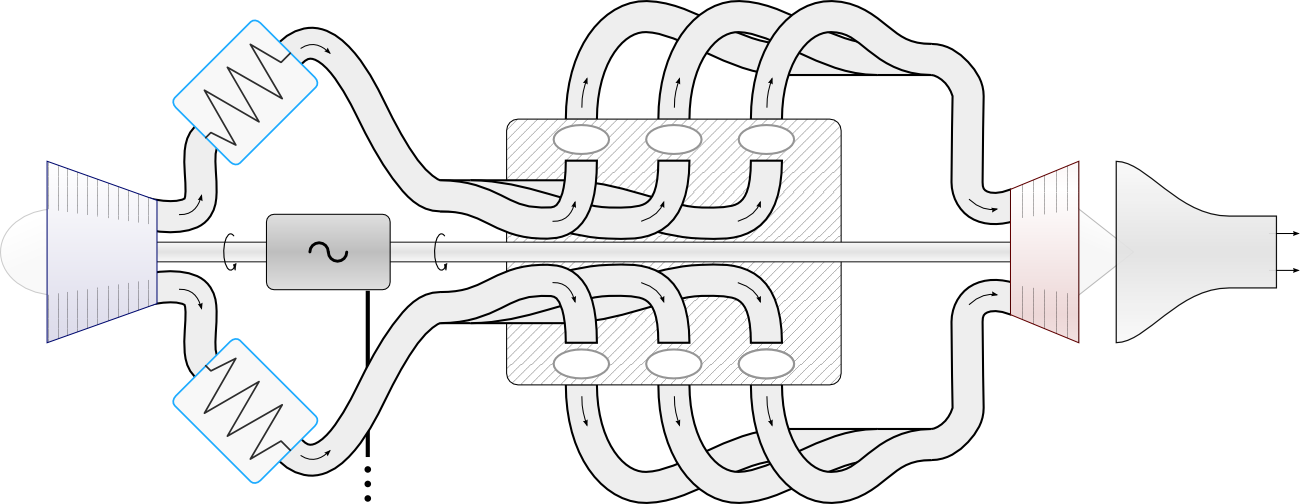
\includegraphics[width=\textwidth]{images/formulaone_engine.png}
			\supercaption{Circuit thermodynamique de l’air d’un moteur de Formule~1 en 2014. L’arbre du turbocompresseur (à gauche) n’est relié ni à celui du moteur six-cylindres (bloc au centre), ni aux roues de la voiture. Toutefois, un moteur/générateur électrique (nommé \textsc{mgu-h}) permet d’en extraire ou d’y apporter de l’énergie électrique. Lors des phases à haute puissance, la puissance de la turbine (à droite) est excédentaire et elle peut être mise à profit pour charger les batteries embarquées ou entraîner les roues avec un moteur électrique. Lors des phases à basse puissance, la turbine est déficitaire et elle peut être entraînée par le générateur pour maintenir le taux de compression et augmenter la réactivité.}%
				{schéma \ccbysa \olivier}
			\label{fig_formulaone_engine}
		\end{center}
	\end{figure}

\atendofhistorysection
